\documentclass{beamer}
\usetheme{Darmstadt}
\usefonttheme[onlylarge]{structurebold}
\setbeamerfont*{frametitle}{size=\normalsize,series=\bfseries}
\setbeamertemplate{navigation symbols}{}
\usepackage{times}
\usepackage{tikz}
\usetikzlibrary{arrows}
\tikzstyle{block}=[draw opacity=0.7,line width=1.4cm]


\title{A Tutorial for {\em Loci}}
\author{Edward Luke}

\begin{document}

\begin{frame}
\titlepage
\end{frame}

%%=============================================================================
\begin{frame}{What is {\em Loci}?}
\begin{itemize}
\item {\em Loci} was originally developed in 1999 as part of National Science Foundation funding supporting the development of advanced multidisciplinary simulation software.
\item {\em Loci} is a sophisticated auto-parallelizing framework that simplifies the task of constructing complex simulation software.
\item {\em Loci} is free software available under the Lesser GNU Public License.
\item The {\em Loci} paradigm is domain specific but powerful and able to capture a wide range of numerical application software.
\end{itemize}
\end{frame}
%%=============================================================================
\begin{frame}{}
\begin{center}
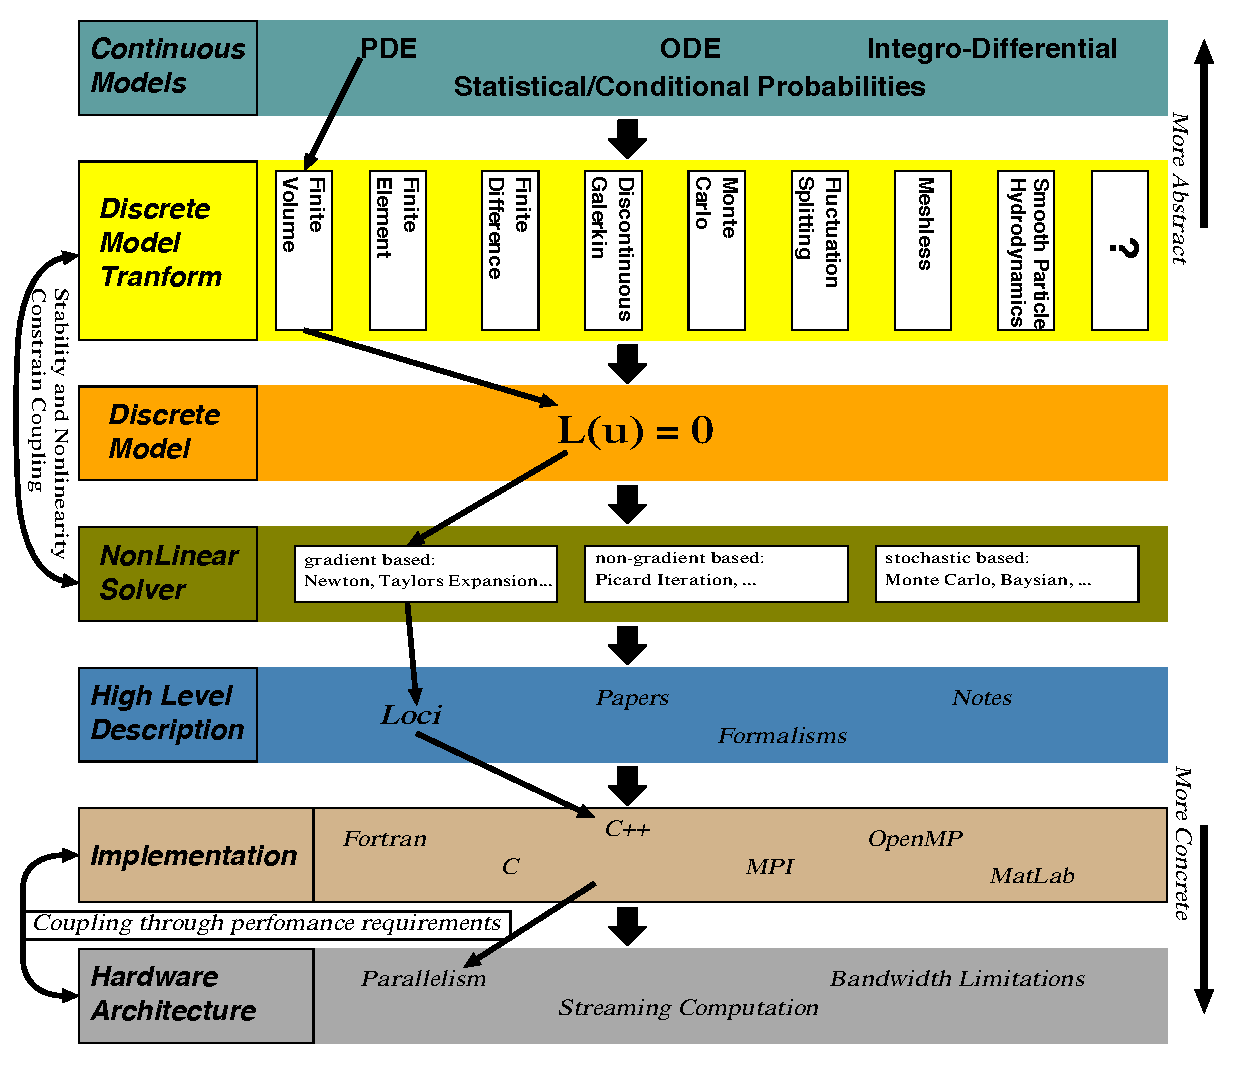
\includegraphics[height=3.2in]{architecture}
\end{center}
\end{frame}
%%=============================================================================
\begin{frame}{{\em Loci} and C++}
\begin{itemize}
\item The {\em Loci} framework is built using the C++ language.
\item A preprocessor ({\tt lpp}) translates {\em Loci} code into the native C++ code
\item Generally users of {\it Loci} only need to know a small amount of C++ to be effective
\item It is possible to interface to external applications and subroutines such as Fortran, however this is an advanced topic and there can be many limitations particularly when executing in parallel
\end{itemize}
\end{frame}

%%=============================================================================
\begin{frame}{What is a declarative programming model?}
\begin{itemize}
\item Most traditional programming models are imperative, that is they are implicitly a list directions that will be performed in the specified order (e.g. How to solve a problem)
\item Declarative programming models work by declaring properties of objects without specifying a recipe for solution.  (e.g. focusing on describing the components that will solve the problem, but not how they will be used)
\item In the declarative approach the assembly of components to solve the problem (the how) is determined by the application of logical inferences from the component specification.
\item Getting used to thinking about problems in a declarative way is the main learning curve for {\it Loci} programming.
\end{itemize}
\end{frame}
%%=============================================================================
\begin{frame}{Declarative Programming in Loci}
\begin{center}
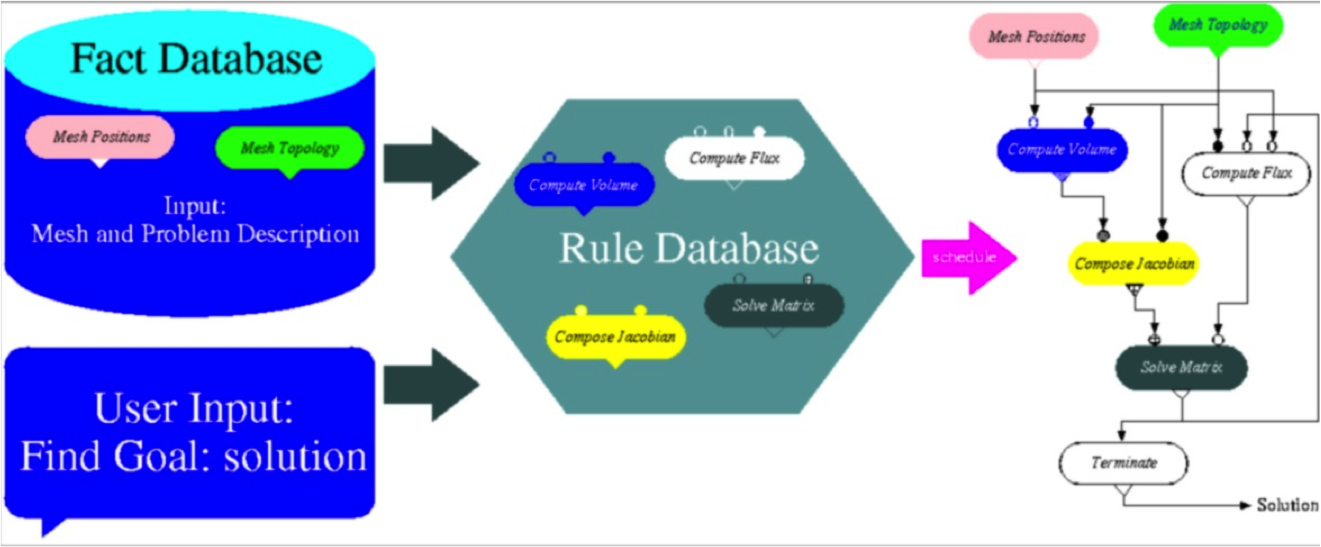
\includegraphics[height=1.5in]{Loci}
\end{center}
\end{frame}
%%=============================================================================
\begin{frame}{{\it Loci} programming preliminaries}
\begin{itemize}
 \item Most {\it Loci} programs will include ``Loci.h''
 \item All Loci programs will need to be initialized and finalized
 \item When using MPI, calls to MPI initialization/finalization are not needed
\end{itemize}
\end{frame}

%%=============================================================================
\begin{frame}[fragile=singleslide]\frametitle{Loci Initialization Code}
\begin{verbatim}
#include <Loci.h>

int main(int argc, char *argv[]) {
   // Initialize Loci
   Loci::Init(&argc, &argv) ;

   // ...
   // Loci Program
   // ...

   // Call finalize for Loci clean up.
   Loci::Finalize() ;
   return 0 ;
}
\end{verbatim}
\end{frame}

%%=============================================================================
\begin{frame}{Entities, Sets, and Sequences}
\begin{itemize}
\item {\tt Entities} are an important concept in {\it Loci}
\item {\tt Entities} are what gives an object an identity in {\it Loci}
\item All entities have a unique identifier and can be used to see which object we are addressing
\item Groups of entities can be represented efficiently as a set called an {\tt entitySet}
\item A group of consecutively numbered entities can be represented in a compact form as an {\tt interval}
\item A ordered sequence of entities is called a {\tt sequence}
\end{itemize}
\end{frame}

\begin{frame}{Entity Sets}
\begin{itemize}
 \item {\tt entitySet} stores sets in a compressed form as a sorted sequence of non-overlapping intervals
 \item Thus the set $A={1,2,3,5,6,7,8,9,10,100}$ will be represented in an {\tt entitySet } as {\tt ([1,3],[5,10],[100,100])}.
 \item The UNIVERSAL set which includes all possible entities is represented with the special notation {\tt ([\#,\#])}.
 \item The EMPTY set is represented as {\tt ()}
 \item Set operations supported are Union ({\tt +}), Intersection ({\tt \&} ), Difference ({\tt -}), Complement ({\tt \textasciitilde}) {\it (show EXAMPLE)}
\end{itemize}
\end{frame}

%%=============================================================================
\begin{frame}{Loci Containers}
\begin{itemize}
\item {\it Loci} provides methods for associating values with entities or associating entities with other entities.
\item The data types that perform this association are called containers.
\item Four main types of containers types include {\tt store}, {\tt parameter}, {\tt map}, and {\tt constraint}
\end{itemize}
\begin{center}
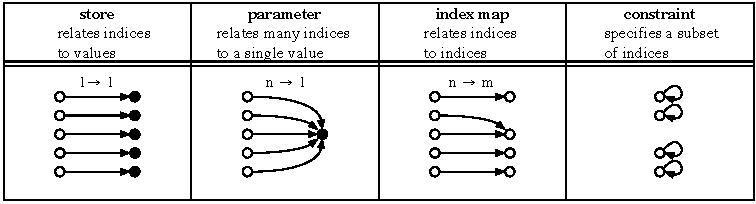
\includegraphics[height=1in]{constructs}
\end{center}
\end{frame}

%%=============================================================================
\begin{frame}{Container Themes}
\begin{itemize}
\item {\tt store<T>} : associates value type {\tt T} with entities
\item {\tt storeVec<T>}: associates n value types {\\ T} with entities
\item {\tt multiStore<T>}: associates variable number of types with entities
\item {\tt Map}: associates 1 entity per entity
\item {\tt mapVec<n>}: associates n entities per entity
\item {\tt multiMap }: associates variable number of entities per entity
\end{itemize}
\end{frame}

%%=============================================================================
\begin{frame}[fragile=singleslide]\frametitle{Container Examples}
\begin{verbatim}
// We create a store of floats
store<float> x ;
// We create a store of std::vectors
store<std::vector<float> > particles ;
// allocate stores x and particles
entitySet alloc_set = interval(1,100) ;
x.allocate(alloc_set) ;
particles.allocate(alloc_set) ;
// initialize the container to the value zero
for( int i=0;i<101;++i) {
  x[i] = 0 ;
  particles[i].push_back(0) ; 
}
\end{verbatim}
\end{frame}

%%=============================================================================
\begin{frame}[fragile=singleslide]\frametitle{Parameter Example}
\begin{verbatim}
param<real> Twall ; // Create wall temperature
Twall = 300 ;
// Constraint Twall to only apply to
// boundary entities (as given)
entitySet wallBoundary = interval(1000,1500) ;
Twall.set_entitySet(wallBoundary) ;
\end{verbatim}
\end{frame}


%%=============================================================================
\begin{frame}[fragile=singleslide]\frametitle{Constraint Example}
\begin{verbatim}
// set inflow constraint
constraint inflow ;
*inflow = entitySet(interval(1,3)) ;
constraint viscous ;
*viscous = EMPTY ; // default not set
if(mu_set) // if viscous set to
  *viscous = ~EMPTY ; // UNIVERSE
\end{verbatim}
\end{frame}

%%=============================================================================
\begin{frame}{The Fact Database}
\begin{itemize}
\item The fact database is a repository for containers in the {\it Loci} Framework
\item The fact database is used to define the initial facts that define the problem setup
\item It is defined by the {\tt fact\_db} data type in {\it Loci}
\item Containers are added to the {\tt fact\_db} using the {\tt create\_fact} member function
\item Containers can be retrieved from the {\tt fact\_db} using the {\tt get\_fact} member function.
\item The fact database does a ``shallow copy'' of the containers.  E.g. the reference to the container (called a {\tt storeRep}) is what is actually stored.
\end{itemize}
\end{frame}

%%=============================================================================
\begin{frame}{What Are Rules?}
\begin{itemize}
  \item Rules are ways to express how one set of facts can be transformed into another set of facts
  \item Rules come in several forms:
\begin{itemize}
\item {\tt default } Default rules are used to define parameters that can be redefined in the vars file (text version of the fact database)
\item {\tt optional} Optional rules tell {\it Loci} about the type of data that may be placed in the vars file.  Since they do not have a default value their existence implies entry in the vars file.
\item {\tt pointwise} A point by point application entity by entity
\item {\tt singleton} Used to perform computations on the single values of parameters
\item {\tt unit} and {\tt apply} are used to form reductions
\end{itemize}
\end{itemize}
\end{frame}
%%=============================================================================
\begin{frame}{The Rule Database}
\begin{itemize}
\item In {\it Loci} rules are used to define transformations from on set of values to another.
\item Users develop applications in {\it Loci} by defining transformation rules (Much more on this later!)
\item The rule database is used to create combined sets of rules that you wish to use to solve your problem.
\item When rules are created in Loci they are automatically added to a list of rules to be processed.  This list is called the {\tt global\_rule\_list}.
\item Rules can be added to the rule database by using the {\tt add\_rules} member function.  Typically this will look like {\tt rdb.add\_rules(global\_rule\_list) ; }
\end{itemize}
\end{frame}

%%=============================================================================
\begin{frame}[fragile=singleslide]\frametitle{The Query}
\begin{itemize}
\item In {\it Loci} applications are developed through making queries to the fact database using a prescribed set of rules.
\item The application that is created as a result of the query depends on the data provide in the fact database (also called the {\it extensive} facts), the provided transformations, and the query.
\item The schedule is generated through a process of generating derived facts ({\it intensive} facts )
\item A schedule is generated by using the {\it makeQuery} call:
\end{itemize}
\begin{verbatim}
// Query for intensive fact 'temperature'
if(!Loci::makeQuery(rdb,facts,"temperature")) 
  cerr << "query failed!" << endl ;
\end{verbatim}
\end{frame}

%%=============================================================================
\begin{frame}{Loci Helper Classes}
\begin{itemize}
\item Loci provides helper classes that can simplify program development
\item Helper classes include:
\begin{itemize}
  \item {\tt Array<T,n>}

    Provides proper semantics for arrays suitable for storing in Loci containers. {\it Do not put C++ arrays in containers!}
  \item {\tt vector3d<T> }

    Provides operators for addition, scalar multiplication, dot and cross products
  \item {\tt vector2d<T> }

    Provides operators for addition, scalar multiplication, dot and cross products
\end{itemize}
\item {\it (Go through example)}
\end{itemize}
\end{frame}
%%=============================================================================
\begin{frame}{The {\tt options\_list} class}
\begin{itemize}
\item For many solvers inputs may be complex and hierarchical.
\item The {\tt options\_list} class is provided to help standardize the input of this sort of data.
\item It is used in most {\it Loci} solvers for inputting boundary condition data.  
\item The general form is a list of assignments of values to named terms called options.
\item In general the value assigned to a name may be a real number, a real number with units, a double, a string, a name, a list, or a function.  
\item Lists or functions may be viewed as a nested options list making the input method very powerful.
\end{itemize}
\end{frame}
%%=============================================================================
\begin{frame}{{\tt options\_list} member functions}
\begin{itemize}
\item {\tt optionExists}Returns a true value of the provided name is in the list of attributes
\item{\tt getOptionNameList}: Returns a list of attributes that have definitions
\item{\tt getOptionValueType}: Returns the type of the data that was assigned to the attribute.  This may be {\tt REAL}, {\tt NAME}, {\tt FUNCTION}, {\tt LIST}, {\tt STRING}, {\tt BOOLEAN}, or {\tt UNIT\_VALUE}.

\item {\tt getOption}: Returns the value associated with the attribute.  The second argument is the returned value and may be the types {\tt bool}, {\tt double}, {\tt string}, or {\tt options\_list::arg\_list}.

\item {\tt getOptionUnits}: This returns a double value in the requested units.
\end{itemize}
\end{frame}

%%=============================================================================
\begin{frame}{A Simple Example: 1-D diffusion}

  Consider the finite volume method solution to this simple one
  dimensional diffusion equation:
\begin{align*}
u_t      & =  \nu u_{xx},~ x \in (0,1), t>0,\\
u(x,0)   & =  f(x),~ x \in [0,1],\\
u_x(0,t) & =  g(t), \mbox{ where } g(0) = f_x(0), \mbox{ and }\\
u(1,t) & =  h(t), \mbox{ where } h(0) = f(1).
\end{align*}

\end{frame}

%%=============================================================================
\begin{frame}{Finite Volume Discretization}
\begin{itemize}
\item Divide the interval $[0,1]$ into  $N-1$ cells by defining $N$ nodes such that $x = \lbrace (i,x_i) | i \in [0, \cdots, N], x_i = i/N \rbrace$
\item Cells are defined by their interfaces to the left and right:
\begin{equation*}
\begin{array}{rcl}
il & = & \lbrace (c,l) | c \in [N+1, \cdots, 2N], l = c-N-1 \rbrace,\\
ir & = & \lbrace (c,r) | c \in [N+1, \cdots, 2N], r = c-N \rbrace.\\
\end{array}
\end{equation*}
\end{itemize}
\begin{center}
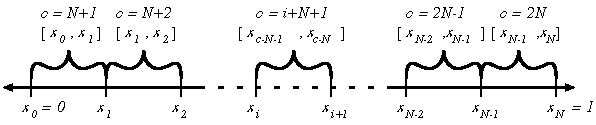
\includegraphics[height=.75in]{one-d}
\end{center}
\end{frame}
%%=============================================================================
\begin{frame}{Indirection Operators}
\begin{itemize}
  \item To implement the finite volume scheme we will need to be able to access values at interfaces, this will be done through composition
  \item For example, to access the left and right nodes of a given cell we could compose the interface maps with the x coordinates with the composition operator:
\begin{equation*}
il\rightarrow x = \lbrace (c,x_l) | (c,l) \in il, (l,x_l) \in x \rbrace.
\end{equation*}
\item Using this operator we can now define other attributes that will be needed to perform numerical integration such as the cell center:
\begin{equation*}
x_c = (ir \rightarrow x + il \rightarrow x)/2.
\end{equation*}
\end{itemize}
\end{frame}

%%=============================================================================
\begin{frame}{Numerical Integration}
\begin{itemize}
\item Using a midpoint rule to numerically integrated in space and a first order explicit Euler integration for time, the numerical solution to the 1-D diffusion equation can be written as:
\begin{equation*}
R(u) = \nu \frac{{ir \rightarrow u_x - il \rightarrow u_x} }{L}
\end{equation*}
\begin{equation*}
u^{n+1} = u^{n} + \Delta t R(u^n)
\end{equation*}
\end{itemize}
\end{frame}

%%=============================================================================
\begin{frame}{Summary of Definitions for Diffusion Problem}
\begin{center}
  \begin{tabular}{|l|l|}
    \hline
    fact      & meaning \\
    \hline
    $\nu$     & given diffusion constant  \\
    $f(x)$     & given initial condition  \\
    $g(t)$     & given left bc \\
    $h(t)$     & given right bc  \\
    $\Delta t$& given time-step  \\
    $x$       & $\lbrace (i,x_i) | i \in [0, \cdots, N], x_i = i/N    \rbrace$\\
    $il$      & $\lbrace (c,l)   | c \in [N+1, \cdots, 2N], l = c-N-1 \rbrace$\\
    $ir$      & $\lbrace (c,r)   | c \in [N+1, \cdots, 2N], r = c-N   \rbrace$\\
    $cl$      & $\lbrace (i,l)   | i \in [1, \cdots, N], l = i+N      \rbrace$\\
    $cr$      & $\lbrace (i,r)   | i \in [0, \cdots, N-1], r = i+N+1  \rbrace$\\
    \hline
  \end{tabular}
\end{center}
\end{frame}

%%=============================================================================
\begin{frame}{Summary of Transformation Rules}
\begin{center}
  \begin{tabular}{|l|l|l|}
    \hline
    Rule  & Rule Signature & Equation\\
    \hline
    Rule 1 & $x_c \leftarrow (ir,il)\rightarrow x $ &    (3.8)\\
    Rule 2 & $ L \leftarrow (ir,il)\rightarrow x $ &    (3.11)\\
    Rule 3 & $u_x \leftarrow (cr,cl)\rightarrow(u,x_c)$ &    (3.13)\\
    Rule 4 & $u_x \leftarrow  h, t, \mbox{constraint}\lbrace 
    \mathrm{dom}(cl) \wedge \neg \mathrm{dom}(cr) \rbrace$ &    (3.14)\\
    Rule 5 & $u_x \leftarrow  g, t, \mbox{constraint}\lbrace 
    \mathrm{dom}(cr) \wedge \neg \mathrm{dom}(cl) \rbrace$ &    (3.15)\\
    Rule 6 & $R\leftarrow \nu,L,(ir,il)\rightarrow u_x$ & (3.16)\\
    Rule 7 & $u^{n+1} \leftarrow u^n, R^n, \Delta t$ & (3.17)\\
    Rule 8 & $u^{n=0} \leftarrow f,x_c,\mbox{constraint}\lbrace(il,ir)\rightarrow
    x\rbrace $ &    (3.19)\\
    \hline
  \end{tabular}
\end{center}
\end{frame}
%%=============================================================================
\begin{frame}[fragile=singleslide]\frametitle{Setting up the fact database}
\begin{itemize}
\item First we create the maps and install them in the fact database (this is the 1-D mesh)

  {\it Go through example online}
\item Then we can setup default parameters as a {\it Loci} program:
\end{itemize}
\begin{verbatim}
// How many nodes
$type N param<int> ;              
// diffusion coefficient
$type nu param<float> ;           

$rule default(N) {  $N=50 ;}
$rule default(nu) {  $nu = 1.0 ;}
\end{verbatim}
\end{frame}

%%=============================================================================
\begin{frame}[fragile=singleslide]\frametitle{Writing the Rules}
Most of the rules translate directly into Loci rules:
\begin{verbatim}
// Rule 1: compute the cell center from node positions
$rule pointwise(xc<-(il,ir)->x) {
  $xc = .5*($il->$x + $ir->$x) ;
}
// Neuman boundary condition at left boundary, ux = h(t)
$rule pointwise(ux<-h), constraint(left_boundary) {
  $ux = $h ;
}
\end{verbatim}
\end{frame}
%%=============================================================================
\begin{frame}[fragile=singleslide]\frametitle{Temporal Integration}
The temporal iteration is then specified
\begin{verbatim}
// Rule 7: initialization of iteration (build rule)
$rule pointwise(u{n=0}<-xc) {
  $u{n=0} = f($xc) ;
}

// Rule 8: time advance using explicit Euler time 
//         integration algorithm
$rule pointwise(u{n+1}<-u{n},dt{n},R{n}) {
  $u{n+1} = $u{n}+$dt{n}*$R{n} ;
}
\end{verbatim}
\end{frame}
%%=============================================================================
\begin{frame}[fragile=singleslide]\frametitle{Terminating The Iteration}
\begin{verbatim}
$rule pointwise(solution<-u{n}),
      conditional(simulation_finished{n}) {
  $solution = $u{n} ;
}
$type max_iteration param<int> ;
$type simulation_finished param<bool> ;

// When is  iteration is complete?
$rule singleton(simulation_finished<-
                              $n,max_iteration) {
   $simulation_finished = ($$n >= $max_iteration) ;
}
\end{verbatim}
\end{frame}

%%=============================================================================
\begin{frame}{Reduction Rules}
\begin{center}
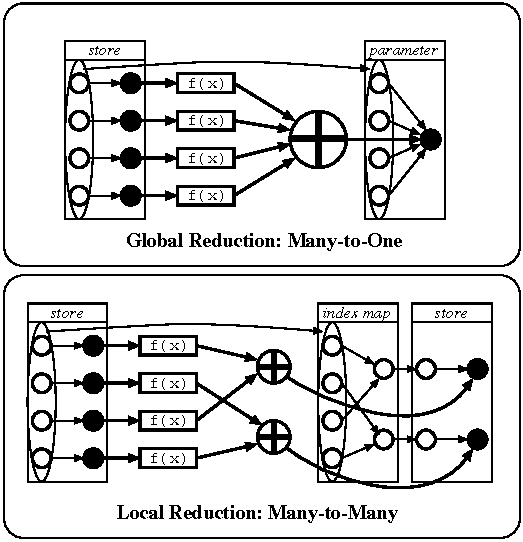
\includegraphics[height=3in]{reduction}
\end{center}
\end{frame}

%%=============================================================================
\begin{frame}{Components of a reduction}
\begin{itemize}
\item An operator that is associative (and commutative)
\item A part that initializes values to the identity of the operator (the unit)
\item A part the produces values that will be combined using the operator (the apply)
\end{itemize}
\end{frame}
%%=============================================================================
\begin{frame}[fragile=singleslide]\frametitle{Stable Timestep Using Global Reductions}
\begin{verbatim}
$type dt param<float> ; // simulation timestep

$rule unit(dt), constraint(UNIVERSE) {
    // largest allowble timestep
   $dt = std::numeric_limits<float>::max() ;
}

$rule apply(dt<-L,nu)[Loci::Minimum] {
    // Stable timestep
    float local_dt = $L*$L/(2.*$nu) ;  
    //  combine local with global
    join($dt,local_dt) ; 
}
\end{verbatim}
\end{frame}
%%=============================================================================
\begin{frame}[fragile=singleslide]\frametitle{Some Pitfalls}
\begin{verbatim}
$rule apply(sum<-terms)[Loci::Summation] {
    // Error!  Result depends on order of sum!
    if($sum < 1) 
      join($sum,$terms) ; 
}
$rule apply(sum<-terms)[Loci::Summation] {
    // OK, result is independent of summing order
    if($terms < 1) 
      join($sum,$terms) ; 
}
\end{verbatim}
\end{frame}
%%=============================================================================
\begin{frame}[fragile=singleslide]\frametitle{More Pitfalls}
\begin{verbatim}
$rule unit(sum), constraint(UNIVERSE){
   // Error, not identity of summation!
   $sum = 1.0 ;
}
$rule apply(sum<-terms)[Loci::Summation] {
   join($sum,$terms) ; 
}
\end{verbatim}
\end{frame}
\begin{frame}{Going to the Implementation}
\begin{itemize}
\item After assembling the rules and facts we can see what kind of application Loci assembles
\item {\it Loci} provides options that allow you to inspect what it has done.  To see what type of program it will generate enter:

{\tt ./heat --scheduleoutput --nochomp}

\item {\it Loci} will also perform different operations depending on what you query.  The default query is ``solution'' but we can also get other schedules by querying other variables:

{\tt ./heat --scheduleoutput --nochomp -q dt}
\end{itemize}
{\it Run and Inspect Example Code}
\end{frame}

%%=============================================================================
\begin{frame}[fragile=singleslide]\frametitle{Loci Reduction Alternative}
\scriptsize
\begin{verbatim}
$rule pointwise(xc<-(il,ir)->x) { $xc = .5*($il->$x + $ir->$x) ; }
\end{verbatim}
Convert to use cl and cr maps instead:
\begin{verbatim}
$rule unit(xc), constraint(geom_cells) {  $xc = 0 ; }
$rule apply(cl->xc <- x)[Loci::Summation] {  join($cl->$xc,.5*$x) ; }
$rule apply(cr->xc <- x)[Loci::Summation] {  join($cr->$xc,.5*$x) ; }
\end{verbatim}
Note: We cannot combine two apply rules into:
\begin{verbatim}
$rule apply((cl,cr)->xc <- x)[Loci::Summation] 
   {  join($cl->$xc,.5*$x) ; 
      join($cr->$xc,.5*$x) }
\end{verbatim}

\end{frame}

%%=============================================================================
\begin{frame}[fragile=singleslide]\frametitle{Parametric Rules}
\scriptsize
\begin{verbatim}
$type cellIntegrate(X) store<float> ;
$type X store<float> ;
$rule pointwise(cellIntegrate(X)<-(il,ir)->X) {
   $cellIntegrate(X) = $ir->$X - $il->$X ;
}

// The 1d diffusion residue
$rule pointwise(R<-nu,cellIntegrate(ux),L) 
   { $R = $nu*$cellIntegrate(ux)/$L ;}
// We find the length of an interval by integrating the position x
$rule pointwise(L<-cellIntegrate(x)) { $L = $cellIntegrate(x) ; }
\end{verbatim}
\end{frame}
%%=============================================================================
\begin{frame}[fragile=singleslide]\frametitle{Parametric unit/apply rules }
\scriptsize
\begin{verbatim}
// A general function for integrating over a cell boundary
$rule unit(cellIntegrate(X)),constraint(geom_cells) {
  $cellIntegrate(X) = 0 ;
}
$rule apply(cl->cellIntegrate(X)<-X)[Loci::Summation] {
  join($cl->$cellIntegrate(X),$X) ;
}
$rule apply(cr->cellIntegrate(X)<-X)[Loci::Summation] {
  join($cr->$cellIntegrate(X),-$X) ;
}
\end{verbatim}
\end{frame}
%%=============================================================================
\begin{frame}[fragile=singleslide]\frametitle{Parametric Time Iteration}
\scriptsize
\begin{verbatim}
// X is the residual, Y is the independent variable
$type EulerIntegrate(X,Y) store<float> ;
$type X store<float> ;
$type Y store<float> ;
$type Y_ic store<float> ;
// Initialize the iteration using the initial conditions
$rule pointwise(EulerIntegrate(X,Y){n=0}<-Y_ic) 
 {  $EulerIntegrate(X,Y){n=0} = $Y_ic ; }

// Collapse iteration when finished
$rule pointwise(EulerIntegrate(X,Y)<-EulerIntegrate(X,Y){n}),
                conditional(eulerTimestepFinished{n}) {
  $EulerIntegrate(X,Y) = $EulerIntegrate(X,Y){n} ; 
}
// Condition for terminating the timestepping algorithm
$rule singleton(eulerTimestepFinished<-$n,max_iteration) 
   {  $eulerTimestepFinished = ($$n >= $max_iteration) ; }
\end{verbatim}
\end{frame}
%%=============================================================================
\begin{frame}[fragile=singleslide]\frametitle{Parametric Time Iteration}
\scriptsize
\begin{verbatim}
// Advance the timestep to the next value
$rule pointwise(EulerIntegrate(X,Y){n+1}<-
                      EulerIntegrate(X,Y){n},dt{n},X{n})  {
   $EulerIntegrate(X,Y){n+1} = $EulerIntegrate(X,Y){n}+$dt{n}*$X{n} ;
}

// Extract independent variableb for residual function 
$rule pointwise(Y<-EulerIntegrate(X,Y)),
     parametric(EulerIntegrate(X,Y)) {
  $Y = $EulerIntegrate(X,Y) ;
}
\end{verbatim}

Note the use of the parametric keyword in last rule!
\end{frame}
%%=============================================================================
\begin{frame}[fragile=singleslide]\frametitle{Euler Integration}
\scriptsize
\begin{verbatim}
// Setup the initial conditions
$rule pointwise(u_ic<-xc) {
  $u_ic = initialCondition($xc) ;
}

// Ask to solve the problem by using the Euler Integration 
// on the function residual, integrating the variable u
$rule pointwise(solution<-EulerIntegrate(R,u)) {
  $solution = $EulerIntegrate(R,u) ;
}
\end{verbatim}
\end{frame}%

%%=============================================================================
\begin{frame}[fragile=singleslide]\frametitle{Schedule}
\tiny
\begin{verbatim}
Iteration Loop{n} {
    eulerTimestepFinished{n}<-$n{n},max_iteration{n} over sequence ([11,20])
    if(eulerTimestepFinished{n}) {
      EulerIntegrate(R,u)<-EulerIntegrate(R,u){n},CONDITIONAL(eulerTimestepFinished{n}) over sequence ([11,20])
    } // if(eulerTimestepFinished{n})

    -------------- Exit of Loop{n}
    if(eulerTimestepFinished{n}) break ;

    cellIntegrate(ux){n}<-CONSTRAINT(geom_cells{n}) over sequence ([11,20])
    u{n}<-EulerIntegrate(R,u){n} over sequence ([11,20])
    ux{n}<-(cl{n},cr{n})->(u{n},xc{n}) over sequence ([1,9])
    ux{n}<-cl{n}->(u{n},xc{n}),ub{n},x{n} over sequence ([10,10])
    cr{n}->cellIntegrate(ux){n}<-ux{n} over sequence ([0,9])
    cl{n}->cellIntegrate(ux){n}<-ux{n} over sequence ([1,10])
    R{n}<-L{n},cellIntegrate(ux){n},nu{n} over sequence ([11,20])
    EulerIntegrate(R,u){n+1}<-EulerIntegrate(R,u){n},R{n},dt{n} over sequence ([11,20])
} // {n}
solution<-EulerIntegrate(R,u) over sequence ([11,20])
\end{verbatim}
\end{frame}
%=============================================================================
\begin{frame}{A Three Dimensional Solver}
\begin{itemize}
\item Next example is an implicit three dimensional heat solver
\item Solves the equation $\frac{\partial}{\partial t} (\rho e) = \nabla \cdot (k \nabla T)$
\item Using standard FVM methods this becomes the discrete equation:
\begin{equation*}
\mathcal{V}_c\frac{Q^{n+1}-Q^n}{\Delta t} = R(Q^{n+1}),
\end{equation*}
\begin{equation*}
R = \sum_{f\in{faces}}
\left[ \mathcal{A}_f k \left(\nabla T_f \cdot \vec{n}_f\right)
\right].
\end{equation*}
\end{itemize}
\end{frame}
%=============================================================================
\begin{frame}{The Implicit Formulation}
\begin{itemize}
\item The residual can be linearized using Taylor's theorem:
\begin{equation*}
R(Q^{n+1}) = R(Q^n) + \frac{\partial R(Q)}{\partial Q} \Delta Q +
O(\Delta t^2),
\end{equation*}
\item which can then be used to form the following implicit form:
\begin{equation*}
\left[ \frac{\mathcal{V}_c}{\Delta t} I - \frac{\partial R(Q)}{\partial Q}\right]\Delta Q =
R(Q).
\end{equation*}
\item For this example we will be using the FVM facilities provided for Loci including mesh readers and a module of operators such as gradients.
\end{itemize}
\end{frame}
%=============================================================================
\begin{frame}{Provided Data Structures}
\tiny
\begin{center}
  \begin{tabular}{|l|l|l|l|}
    \hline
    Fact  & Type & Location & Description\\
    \hline\hline
    {\tt pos} & {\tt store<vector3d>} & nodes & Node Positions\\
    {\tt face2node} & {\tt multiMap} & faces & Nodes that form a
    face\\
    {\tt cl} & {\tt Map} & faces & cell left of face\\
    {\tt cr} & {\tt Map} & faces & cell right of face\\
    {\tt ref} & {\tt Map} & boundary faces & map to referring category\\
    {\tt boundary\_names} & {\tt store<string>} & boundary categories & boundary category name\\
    {\tt geom\_cells} & {\tt constraint} & physical cells & set of actual cells\\
{\tt cells} & {\tt constraint} & cells & cells including ghost cells\\
    \hline
  \end{tabular}
\end{center}
\begin{center}
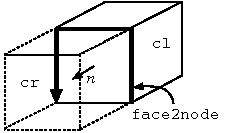
\includegraphics[height=1in]{face}
\end{center}
\end{frame}
%%=============================================================================
\begin{frame}[fragile=singleslide]\frametitle{database setup}
\scriptsize
\begin{verbatim}
rule_db rdb ; // Create the rule database
rdb.add_rules(global_rule_list) ; // Add any user defined rules ;
// Load in the finite-volume module called "fvm"
Loci::load_module("fvm",rdb) ;

// First read in user defined facts
string varsFile = "heat.vars" ;
facts.read_vars(varsFile,rdb) ;

// Next read in the grid file
string file = "heat.xdr"
if(!Loci::setupFVMGrid(facts,file)) {
  cerr << "unable to read grid file '" << file << "'" << endl ;
  Loci::Abort() ;
}
// Deconstruct boundary_conditions variable
setupBoundaryConditions(facts) ;
// Setup Matrix
createLowerUpper(facts) ;
\end{verbatim}
\end{frame}
%%=============================================================================
\begin{frame}{Matrix Setup}
\begin{center}
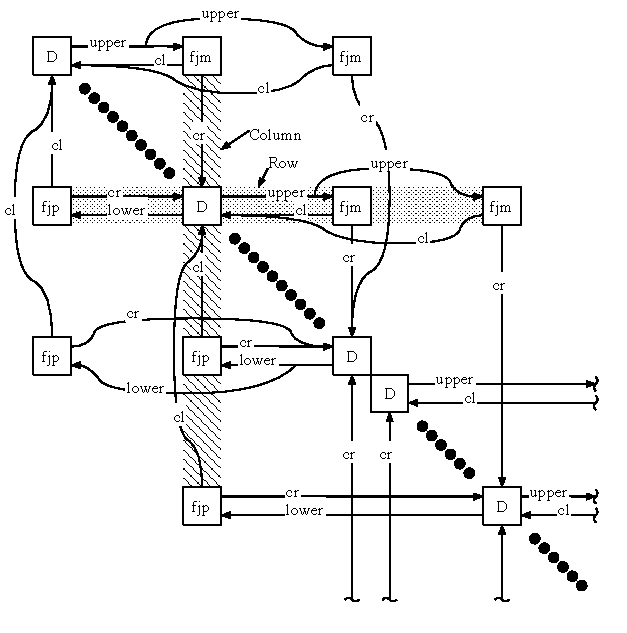
\includegraphics[height=3in]{mat}
\end{center}
\end{frame}
%%=============================================================================
\begin{frame}{Matrix Cell View}
\begin{center}
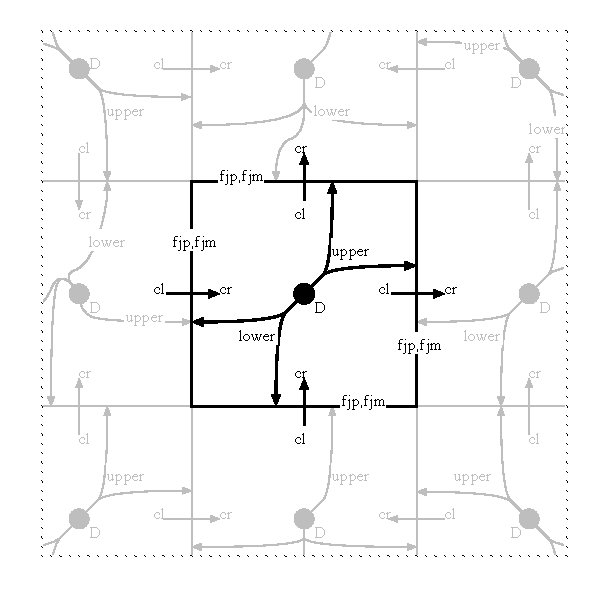
\includegraphics[height=3in]{cell}
\end{center}
\end{frame}
%%=============================================================================
\begin{frame}[fragile=singleslide]\frametitle{Boundary Condition Rule Setup}
\scriptsize
\begin{verbatim}
// Extract Twall from boundary condition options
$rule pointwise(Twall<-BC_options),constraint(Twall_BCoption) {
  $BC_options.getOptionUnits("Twall","kelvin",$Twall) ;
}
// Temperature at wall set to specified condition
$rule pointwise(temperature_f<-ref->Twall),constraint(specified_BC) {
  $temperature_f = $ref->$Twall ;
}
// Handle Boundary Conditions
// Adiabatic Wall, qdot = 0, grad(temperature) = 0
$rule pointwise(adiabatic::qdot),constraint(adiabatic_BC) {
  $qdot = 0 ;
}
\end{verbatim}
\end{frame}

%%=============================================================================
\begin{frame}[fragile=singleslide]\frametitle{Residual Evaluation}
\scriptsize
\begin{verbatim}
// Compute the heat flux through faces
$rule pointwise(qdot<-conductivity,grads_f(temperature),area) {
  $qdot = $area.sada*$conductivity*dot($grads_f(temperature),$area.n) ;
}
// Add up contributions from all faces, only define qresidual for geom_cells
$rule unit(qresidual),constraint(geom_cells) {
  $qresidual = 0 ;
}
// Add to left cell
$rule apply(cl->qresidual<-qdot)[Loci::Summation],
  constraint(cl->geom_cells) {
  join($cl->$qresidual,$qdot) ;
}

// Add to right cell, note sign change due to normal pointing into cell
$rule apply(cr->qresidual<-qdot)[Loci::Summation],
  constraint(cr->geom_cells) {
  join($cr->$qresidual,-$qdot) ;
}
\end{verbatim}
\end{frame}
%%=============================================================================
\begin{frame}[fragile=singleslide]\frametitle{Residual Evaluation: Missing Part}
\scriptsize
\begin{verbatim}
// Compute boundary temperatures for gradients
// adiabatic,  dT/dx = 0, so copy temperature from cell to face
$rule pointwise(temperature_f<-cl->temperature),constraint(adiabatic_BC) {
  $temperature_f = $cl->$temperature ;
}

// Temperature Specified Wall
$rule pointwise(temperature_f<-ref->Twall),constraint(specified_BC) {
  $temperature_f = $ref->$Twall ;
}
\end{verbatim}
\end{frame}

%%=============================================================================
\begin{frame}[fragile=singleslide]\frametitle{Matrix Preliminaries, derivatives}
\tiny
\begin{equation*}
\frac{\partial \dot{q}}{\partial Q_l} = \frac{\partial \dot{q}}{\partial T_l} \frac{\partial T_l}{\partial Q_l} = \frac{\mathcal{A}_f k }{(\vec{x}_l-\vec{x}_r)\cdot \vec{n}_f}\frac{\partial T_l}{\partial Q_l},
\end{equation*}
and
\begin{equation*}
\frac{\partial \dot{q}}{\partial Q_r} = \frac{\partial \dot{q}}{\partial T_r} \frac{\partial T_r}{\partial Q_r} = -\frac{\mathcal{A}_f k }{(\vec{x}_l-\vec{x}_r)\cdot \vec{n}_f}\frac{\partial T_r}{\partial Q_r}.
\end{equation*}

\begin{verbatim}
// Derivative of flux from left side
$rule pointwise(dqdotdQl<-conductivity,(cl,cr)->cellcenter,area,cl->dTdQ) {
  real distance = dot($cl->$cellcenter-$cr->$cellcenter,$area.n) ;
  $dqdotdQl = $area.sada*$conductivity*$cl->$dTdQ/distance ;
}

// Derivative of flux from right side
$rule pointwise(dqdotdQr<-conductivity,(cl,cr)->cellcenter,area,cr->dTdQ) {
  real distance = dot($cl->$cellcenter-$cr->$cellcenter,$area.n) ;
  $dqdotdQr = -$area.sada*$conductivity*$cr->$dTdQ/distance ;
}
\end{verbatim}
\end{frame}
%%=============================================================================
\begin{frame}[fragile=singleslide]\frametitle{Matrix Assembly}
\tiny
\begin{verbatim}
// To compute the diagonal term, we first must sum the diagonal
// contributions from the flux derivatives.
$type sumDiagonal store<real> ;

// Add up diagonal contributions from flux derivatives
$rule unit(sumDiagonal), constraint(geom_cells) { $sumDiagonal = 0 ;}

// Add contribution from face to left cells
// (e.g. d R(Ql,Qr)/d Ql goes to diagonal of the left cell)
$rule apply(cl->sumDiagonal<-dqdotdQl)[Loci::Summation],
  constraint(cl->geom_cells) {
  join($cl->$sumDiagonal,$dqdotdQl) ;
}

// Add contribution from face to right cells 
// (e.g. d R(Ql,Qr)/d Qr goes to diagonal of the right cell)
// Note sign change due to normal pointing into the cell
$rule apply(cr->sumDiagonal<-dqdotdQr)[Loci::Summation],
  constraint(cr->geom_cells) {
  join($cr->$sumDiagonal,-$dqdotdQr) ;
}
$rule pointwise(heat_D<-sumDiagonal,deltaT,vol) {
  $heat_D = $vol/$deltaT - $sumDiagonal ; 
}
\end{verbatim}
\end{frame}
%%=============================================================================
\begin{frame}[fragile=singleslide]\frametitle{Matrix Assembly}
\scriptsize
\begin{verbatim}
$rule pointwise(heat_B<-qresidual) {
  $heat_B = $qresidual ;
}
// Compute matrix lower term from flux derivatives
// Note, we are subtracting del R/del Q in the matrix so there is an
// extra sign change here
$rule pointwise(heat_L<-dqdotdQl) {
  $heat_L = $dqdotdQl; 
}

// Compute matrix upper term from flux derivatives
$rule pointwise(heat_U<-dqdotdQr) {
  $heat_U = -$dqdotdQr;
}

// Solve linear system described by heat_B, heat_D, heat_L, heat_U
$rule pointwise(deltaQ<-petscScalarSolve(heat)) {
  $deltaQ = $petscScalarSolve(heat) ;
}
\end{verbatim}
\end{frame}

%%=============================================================================
\begin{frame}[fragile=singleslide]\frametitle{Time Integration}
\scriptsize
\begin{verbatim}
// Initial Conditions
$rule pointwise(Q{n=0}<-Density,Cp,T_initial) {
  $Q{n=0} = $Density*$Cp*$T_initial ;
}
// Advance the timestep using linear system solution
$rule pointwise(Q{n+1}<-Q{n},deltaQ{n}), constraint(geom_cells) {
  $Q{n+1} = $Q{n}+ $deltaQ{n} ;
}
// Determine when we will finish timestepping
$rule singleton(finishTimestep<-$n,stop_iter) {
  $finishTimestep = ($$n > $stop_iter) ;
}
// Collapse to solution when we are finished iterating
$rule pointwise(solution<-Q{n}),conditional(finishTimestep{n}),
  constraint(geom_cells) {
  $solution = $Q{n} ;
}
\end{verbatim}
\end{frame}
%%=============================================================================
\begin{frame}[fragile=singleslide]\frametitle{Closing the Equations}
\scriptsize
\begin{verbatim}
// Compute temperature from energy
$rule pointwise(temperature<-Q,Density,Cp), constraint(geom_cells) {
  $temperature = $Q/($Density*$Cp) ;
}
// Compute transformation derivative from temperature to Q
$rule singleton(dTdQ<-Density,Cp) {
  $dTdQ = 1./($Cp*$Density) ;
}
\end{verbatim}
\end{frame}
\begin{frame}{Running the case}

{\it Run the case!}
\end{frame}
% \begin{frame}[fragile=singleslide]\frametitle{Loci Initialization Code}
% \begin{verbatim}
% \end{verbatim}
% \end{frame}

\end{document}
